\chapter{Background Literature}
\label{BackgroundLit}

\section{Introduction}
\label{BL:Intro}
This chapter reviews extant literature surrounding the design and deployment of technologies for and with people with dementia, the current public perspective of dementia, and how people with dementia are recognised and contribute to research and design. It reviews topics relating to the research questions: participation and technology development with people with dementia; ethical complexities researchers face in everyday dementia interactions; representation of dementia; and the different stakeholders and interests that are designed for (or neglected). This chapter is split into three subsections that ultimately provide four areas of investigation that the thesis examines.

Part one first describes researchers view of dementia as moving from a biomedical to a more person-centred view. I then describe how this model shifted perspectives on dementia in early HCI work to move towards a user-centred approach for design. From here, I introduce literature from HCI in the context of dementia to unpack in which people with dementia are represented and designed for in different stages of technology development. This section describes relational approaches to collaborating with people with dementia as opposed to approaches more commonly taken within research ascribing to the biomedical model. Additionally, it provides insights into researchers' experience of ethical complexities when collaborating with people with dementia. For instance, this section examines the need for researchers to build relationships with participants, carefully reshaping approaches to involve and represent various stages of dementia, and navigate gatekeepers and other diverse stakeholders who are part of the care ecology. In part two, I review how researchers recruit, involve and represent the experiences and views of dementia. From here, I examine the types of ethical dilemmas, public perceptions of dementia and fitting co-design to co-creation for the involvement of later stages of dementia.

Finally, I conclude the literature review by articulating four avenues of investigation that might broaden our understanding of how to design and develop technology for and with people with dementia. This section considers: a) attending to mutual collaborative relationships; b) representation of technology and dementia from a designer/developer perspective; c) ethical practice in HCI in the context of dementia; and d) promoting learning around dementia and technology.

\section{Moving away from a biomedical deficit model of dementia}
\label{BL:DementiaHCI}
Over the last 40 years, researchers and care practitioners have seen our understanding of dementia evolve to position and represent the person with dementia. What was once a biomedical stance has gradually moved towards one that considers the socio-political and individual experiences of dementia \citep{bellass_broadening_2019}. In the early years of dementia research, the biomedical view was viewed through its neurodegenerative condition, emphasising the person's abilities, memory, judgement and communication. By taking a biomedical approach, researchers recognised the potential strain on care partners; improvements in identifying and diagnosing dementia; development of medication to reduce symptoms of dementia; and recommendations on dementia care for policymakers \citep{doi:10.1080/13607863.2019.1693968}. Moreover, given that there are still no known treatments to stop the progression of dementia, there has been significant work and research funding into understanding the causes of the neurodegenerative condition \citep{bature_signs_2017}.

However, several negative consequences arose from the biomedical lens that have had significant social ramifications on people with dementia. First, the biomedical view promotes a view of `loss of self' \citep{ryan_dementia_2009}. Early work by \cite{cohen_loss_1986} believed that people living with dementia \textit{``must eventually come to terms with ... the complete loss of self''}. Views of dementia that see it as a state of deficiency often place the person with dementia as a passive \textit{`patient'} that focuses on being treated rather than living well with dementia. As dementia progresses, it often adds conflict between the person with dementia's surroundings as they become unfamiliar, and in turn, causes difficulties coexisting in places with others, such as a family home or a workplace \citep{langdon_making_2007}. Finally, as we live in a society that places great value on cognitive ability, many believe that people with dementia are poor at social contact, which then prohibits many of them from interacting with people with dementia at all \citep{killick_communication_2001}. For instance, \cite{mukadam2012reducing} reported that public stigma resulted in stereotypes which in turn, caused people with dementia to be \textit{``judged based on stereotypes rather than individual merit, [which] unsurprisingly, may cause distress, and the experience of stigma is associated with
lower self-esteem, disrupted family relationships
and adversely affects social contact, housing and
employment opportunities''}.

From the early 1990's, researchers began to contest the limitations of the biomedical stance by highlighting that the quality of life of the person with dementia is determined not only by neuropathology but also by how they are perceived in society, personal history, and interactions and desires \citep{o2007personhood}. Since the 1990's, there is growing literature indicating that an approach to care that supports inclusion, trust and the individual's personhood may delay or reduce several negative consequences that may develop with dementia. Tom Kitwood, one of the more prominent researchers to tackle the biomedical view, defined the personhood of the person with dementia as \textit{``the standing or status that is bestowed upon one human being, by others, in the context of relationship and social being''} \citep[p.8]{kitwood1997dementia}. Instead of seeing the person with dementia through their disease, Kitwood challenged this by centring the personhood of the individual by personalising care, paying attention to their relationships and maintaining decision-making by acknowledging the person's remaining abilities. The approach has brought forth the sharing of people's experiences with dementia that has redefined how we speak and involve people with dementia in research. The focus on lived experiences has not only demonstrated the importance of individuality in care, but has created a cultural and positive change towards those who have recently been diagnosed with dementia by addressing the anxiety of the varying symptoms of dementia - also known as `dementia worry' \citep{kessler_dementia_2012}.

An integral part of HCI work builds on personhood approaches where design and technology advancements have moved towards improving quality of life, supporting inclusion, evoking emotion and engaging through creativity to help foster heightening subjective wellbeing. While many creatively oriented technologies have relied on the person's ability to articulate past events or configure dementia as a series of problems, as researchers have moved towards the inclusion of the voices of people living with dementia, recent HCI research has similarly begun to question how to position people with dementia in the designing of technology appropriately. With this in mind, the following subsections review HCI literature, in the context of dementia that investigates the types of technologies, design and participatory approaches that researchers use in the domain.

\subsection{Moving to a user-centred approach}
\label{BL:Tech}
Within HCI, early work in dementia focused on the role of assistive technology to support independent living for people with dementia. \citeauthor{bharucha2009intelligent}'s (\citeyear{bharucha2009intelligent}) review of assistive technology applications highlighted an array of different sensors and devices built to compensate for physical and cognitive deficits of people with dementia. For instance, the authors mentioned one typed of device, GPS trackers, to tackle the problem of `wandering'. The term wandering derives from categorising particular `behaviours' in people with dementia where individuals may get lost or forget where they were going. While walking is beneficial for the person with dementia, the action of `wandering' has often been associated with potential harm and emotional stress for the person with dementia and their care partners \citep{robinson2007balancing}. As seen in \citeauthor{bharucha2009intelligent}'s (\citeyear{bharucha2009intelligent}) work, these early studies focusing on `problems' caused by dementia are often guided by family and professional care staff instead of people with dementia. Similarly, early work in care home architecture \citep{torrington2006has}, care processes \citep{rabins2006practical} and creative therapy \citep{schmitt2006creative} prioritised those without dementia in the development processes. This has resulted in prior products and services failing to represent the desires and needs of people with dementia, in turn causing a lack of uptake and ownership of technology design \citep{gibson2019personalisation}. 

Alternatively, \cite{robinson2009keeping} introduced more user-centred design methods that have promoted personhood through the technologies we design. In the authors' study, they ran a series of user-centred design sessions with people with dementia and their carers to design and develop a set of prototypes to facilitate independence for the person with dementia and centre their voices in the design process. The authors' findings highlight opportunities to involve people with dementia in technology's design and iterative stages. Through the series of workshops, the team worked closely with participants with dementia to iterate on the design of two devices (armband and electronic notepad) that demonstrated that these devices are more accepted by people with dementia when they are relevant to their needs and desires. Again, the authors  remarked that adoption would require the support of user-friendly interfaces for carers to ensure that the person with dementia used the assistive technology. 

\cite{wallace_design-led_2013} extend the user-centred approach by turning to a more experiential approach known as experience-centred design (ECD). Through this approach, ECD focuses on \textit{``an understanding of individuals, their concerns, desires, aspirations, values, and experiences''} \citep{morrissey_value_2017} constructed by dialogue, storytelling, and reflection. Their paper, `A Design-led Inquiry into Personhood in Dementia' \citep{wallace_design-led_2013}, related working closely with a married couple (John and Gillian), where Gillian had recently been diagnosed with dementia, to design pieces of digital jewellery to support her personhood. To involve and empathically engage the couple in the design process of the jewellery, the study was carried out as a piece of research through design (RTD). This is a way of carrying out research: it is the practice of design used to address problems with a sense of complexity and no current solution. The approach seeks to address the problem within its current situation \citep{zimmerman_research_2007}. It is generally acknowledged to involve end users within the design process to address and reflect on problems within the associated design space. Through the creation of digitally mediated experiences, the interactions and design decisions provided \cite{wallace_design-led_2013} with insights into the experiences of the married couple in order to keep the experience alive in digital jewellery. While they highlighted the value in this approach to provide insights and understandings into the experiences of people with dementia, exploratory studies that build technology may fall short in supporting the longevity of the technology, resulting in complexities for the participants in the long term. 

\cite{meurer_designing_2018} expanded on issues of `innovation' in research, which hinders opportunities to create sustainable technology - causing frustrations for participants when they depend on a prototype that they can no longer fix due to reaching the end of the study funding. \cite{vines_our_2017} described frustrations while using Google Glass in its beta stages, where participants would encounter many software bugs. These bugs ranged from poor battery life to Google Glass updating itself while in use. With these additional complexities, there are opportunities to consider ways to reinforce the robustness and longevity of technology when the project ends. To achieve this, perhaps research may perhaps focus on building genuine connections with the participants that mirrors \citeauthor{wallace_design-led_2013}'s (\citeyear{wallace_design-led_2013}) work, or maybe building communities of people with dementia, designers and developers who may support the longevity of the technology. To examine how people with dementia contribute to the different stages of design and technology development, the following section explores how researchers facilitate, build relationships and creatively design methods to ensure that people with dementia can contribute to research and be recognised for their contribution.

\section{The stages of participation in technology development}
\label{BL:StagesofTech}

\begin{figure}[htp]
    \centering
    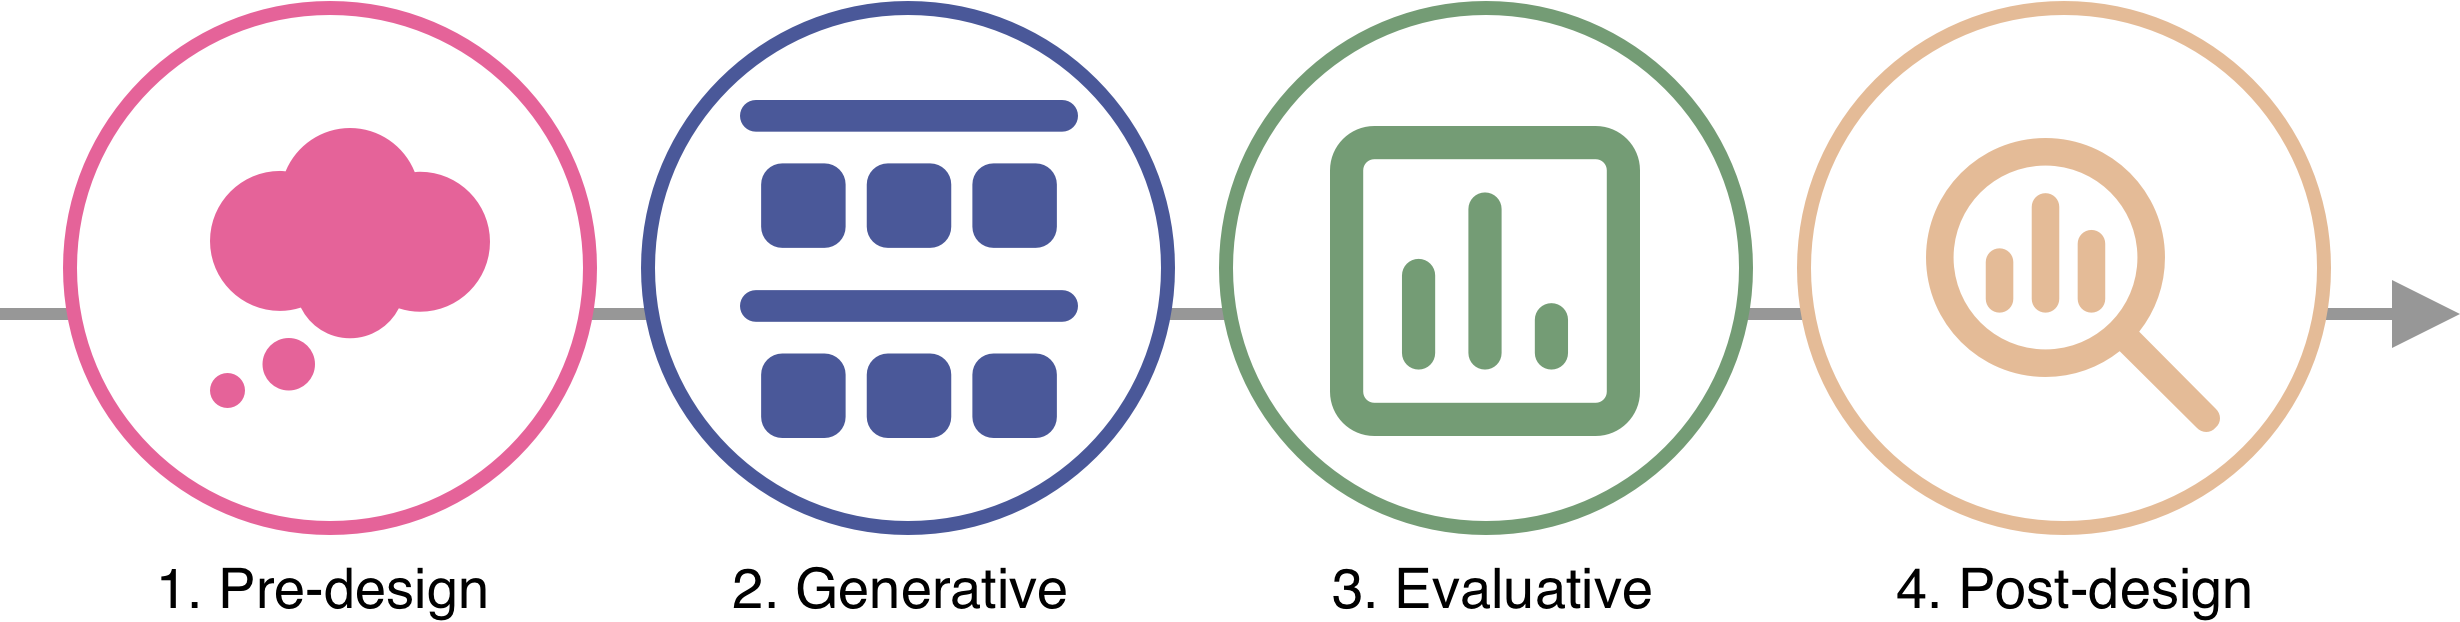
\includegraphics[width=0.8\linewidth]{Images/ChapterTwo/PhasesOfTech.png}
    \caption{Four phases of tech development \citep{suijkerbuijk_active_2019}}
    \label{fig:PhasesOfTech}
\end{figure}
In a recent systematic review of developing supporting technologies for and with people with dementia, \cite{suijkerbuijk_active_2019} categorised technology development into four phases (seen in figure \ref{fig:PhasesOfTech}):

\begin{itemize}
    \item \textbf{Pre-design}: Explores the experiences of the people for whome designers are designing.
    \item \textbf{Generative}: A series of co-design activities to generate ideas for new designs.
    \item \textbf{Evaluative}: Prototypes are tested, and iterative development occurs.
    \item \textbf{Post-design}: The technology is deployed and tested by participants.
\end{itemize}

During these phases, the authors report that the involvement of people with dementia varies from phase to phase. For instance, the evaluative phase is often seen in dementia research as testing prototypes with people with dementia as behaviour and interactions can easily be observed. As such, this section is split into three sub-sections: a) Ways researchers \textit{facilitate participation}; b) Asking at \textit{what stages are people with dementia involved?}; and c) How researchers must build \textit{researcher-participant relationships} when meaningfully engaging with people with dementia.

\subsection{Facilitating participation}
\label{BL:SupportParticipation}
In order to facilitate participation for people with dementia, researchers have involved care partners and adopted ethnographic approaches to build a richer understanding of the person with dementia to ensure they are represented in the design process, and have designed cultural probes to support conversation. Researchers have used several strategies to overcome the challenges of involving people with dementia in the generative process, which typically consists of a set of co-design or participatory activities to generate ideas for new designs \citep{suijkerbuijk_active_2019}. \cite{mayer2013lessons} designed a set of games that embedded `memory' and puzzles as part of the process. By inviting a group of people with dementia to the focus group, the `memory' game cards prompted topics for conversation. The authors described initial challenges in being flexible with how the card game was used. For instance, if participants found the puzzle difficult, the researchers would adjust the difficulty level to ensure everyone could participate. Additionally, inviting people with dementia to the generative design process to generate new design ideas requires researchers to be flexible in their protocol. This may mean changing conversation topics, changing to different activities or even scrapping an activity altogether.

Similarly, \cite{span2015interactive} described the necessity for researchers to be flexible and invest time in understanding their participants. The authors recruited 23 people with mild to moderate dementia to co-design an interactive web tool, DecideGuide, to facilitate shared decision-making in their care networks. To co-design the tool's content, participants took part in semi-structured interviews and focus groups. Within these techniques, participants would engage with decision topics, personal values, and opportunities and challenges of decision-making. However, while the authors reported that the participants engaged with meaning in the research, this took a considerable time investment by the researchers and the participants. For example, the researcher took time into getting to know the participants, upskill them on the use of the technology, and adjusting session flow to the participant's pace. In this way, researchers are required to be flexible in the early stages of design to ensure participants are listened to and supported in sharing their decisions and opinions.

\cite{houben_foregrounding_2019} designed a musical probe to facilitate the exploration of personal experiences of people in early to moderate stages of dementia. In this study, the authors developed a tangible design artefact, the dementia soundboard, that provides meaningful activity and conversation between people with dementia through discovery and exploration of everyday sounds played from the device. While the artefact primarily prompted participants to share childhood memories and reminisce about loved ones, the authors illustrated ways in which the soundboard led to participants asking questions about the research aims, the potential outcomes, how the soundboard was built and feedback on how it might fit into the individual's lives. Similarly, \cite{brown2014using} developed a series of cultural probes to document the lives of care partners and people with dementia. Through cameras, diagrams, postcards and maps, the researchers provided tools to allow participants to capture their data and communicate in more creative and visual ways. These examples offer alternative possibilities for people with dementia to participate that move away from the more traditional approaches such as interviews and focus groups. 

With this in mind, supporting people with dementia in participation requires careful consideration for ways to facilitate and be mindful of the person with dementia's abilities. While the multiple studies focus on the early to mid-stages of dementia, the design of probes or physical materials to facilitate conversation makes it potentially more manageable for people with dementia to be involved and articulate their opinions. Furthermore, multiple studies involved care partners and other members of the ecology of care in supporting decision-making processes. This research highlights several opportunities for HCI work to ensure the person with dementia drives the experience and contributes to the research in any way, shape or form possible.

\subsection{At what stages are people with dementia involved?}
\label{BL:DevelopmentPhases}
From \citeauthor{suijkerbuijk_active_2019}'s (\citeyear{suijkerbuijk_active_2019}) review, the involvement of people with dementia varied significantly through the four phases of technology development. The authors reported that in HCI studies, the involvement of people with dementia in the evaluative phase is unsurprisingly prevalent, this is, the stage where prototypes are tested, and iterative development occurs. This is due to the evaluative phase not requiring people with dementia to reflect on their experiences or provide feedback on the type of ideas they may require. 

For instance, \cite{unbehaun_facilitating_2018} described a 16-month participatory study in a daycare centre where the authors developed a series of exergames to gamify the resident's cognitive training plan. During their prototyping phase, the team deployed several exergame prototypes in the daycare centre for 12 months. To evaluate the prototype, the researchers observed and measured participants using the system alongside informal feedback sessions while residents played the exergames. The group of 14 individuals with dementia ranged from mild to moderate stages of dementia. Throughout the 12 months of observing and evaluating the prototype, the authors reported how useful it was to iteratively tweak the system to the needs, problems and expectations of their participants throughout the study. Furthermore, by spending a considerable amount of time observing these deployed prototypes in their natural settings, the authors highlighted how they could examine the needs of all relevant stakeholders to ensure that the final prototype would not only consider unique ways to follow the cognitive training plan, but to guarantee that set-up and engagement for the care partners was implemented. 

\cite{lindsay_empathy_2012}, in `Empathy, participatory design and people with dementia', described working with early to moderate stages of dementia when running workshops and interviews. During their exploratory phase, which engaged with how technology might support the independence of `getting out and about', the researchers ran a set of participatory design workshops, informal meetings and interviews that focused on relational approaches to building relationships between the researchers and people with dementia and involvement of care partners. Care partners would assist in communication to support participation if it became a challenge for the person with dementia. However, the authors highlighted the challenges of carrying out this sort of research where distinguishing the person with dementia's interests, views and opinions from those of their care partner. In response, the authors suggested that researchers might require longer-term projects and build a rapport with people with dementia throughout the study to ensure the participant has adequate time to contribute.

When working with advanced stages of dementia, \cite{foley_struggle_2019} reported on taking a two year ethnography within a care home to understand the ways in which technology and design can enrich their lives. Here, the authors drew on recognition theory to support collaborative actions and sense-making through the design process. This could be through the use of a participants individual items with person meaning, such as a participant and their scarf; or the designing of tools or probes as a way to encourage and support conversation. From working closely with the members at the care home, the authors developed a conversational aid game called Printer Pals, a media-centred print based quiz game \citep{foley_printer_2019}. 

By the authors spending considerable amount of time with the care home residents, the observations provided insights into the type of potential features and ways technology might support social activities between the residents. For instance, design considerations such as the speed of the printer were influenced by prior ethnography work to ensure everyone had time to participate. For the evaluative phase, the authors `cheap' workable prototypes made from cardboard and a Raspberry Pi focus on the interactions within the care home rather than the look. Using observations and feedback, they redesigned Printer Pals to consider the aesthetics and haptic qualities among additional accessibility features such as altering the volume for those who are hard of hearing. In these examples, while people with dementia were not directly involved in generating ideas for what the research team would develop, through getting to know the residents and observing the relationships and interactions within the care home where the technology would be placed, provided the authors the confidence to make design features on behalf of residents that recognise the shared interests and caring relationships.

Likewise, \cite{lazar2018making} presented an analysis of the ways art therapy could support people with complex communication needs in the early stages of technology development. Working with 22 art therapists, the work emphasised the use of art materials and artwork as a creative process as opposed to relying on verbal interactions with people with dementia. Through the use of creative and meaning-making, the facilitation provided a safe environment where people with dementia could express themselves and respond to issues that matter to them. The authors argued that this alternative form of communication requires alternatives to how researchers convey and represent the findings. For instance, the authors suggest using pictorials at conferences, art exhibitions, and visual thinking galleries.

\subsection{Researcher-participant relationships}
\label{BL:Trust}
Returning to \cite{lindsay_empathy_2012}, the authors described the necessity of building relationships with participants where research engagement is carried out over several workshops. Several HCI researchers have used ethnographic approaches to understand the everyday lives of people with dementia and their interactions with technology. This often requires building relationships between the researchers and the community they observe. For example, the ethnographic work of \cite{lazar_supporting_2017} involved two years of fieldwork at an art therapy programme observing art therapists and adults with dementia, which resulted in the design of a photo-sharing tool. Through a series of workshops and analysis of ethnographic work, the tool aimed to provide people with dementia with ways to share their artwork with friends and family to support their agency. Similarly, \cite{bell2019collaborative} described the necessity of building rapport and trust with their participants when working with younger onset people with dementia to create a safe space for sharing personal stories. For instance, the authors mentioned a one-to0three-month design phase about getting to know the individual participant. This was carried out through social activities, regular visits to their homes, and non-research related texts and phone calls to get to know the person and not just their dementia. The authors reported sharing stories with the participants regarding her connection and experiences with dementia in her family. 

Additionally, \cite{foley_student_2020} talked about students building trust and relationships through co-design methods with care home residents to support meaningful exchange and interaction by developing life story work. In this work, eight undergraduate psychology students volunteered in a residential care unit over two years, working closely with residents with later stages of dementia. The first author describes how, initially, they would put \textit{``considerable input in terms of facilitating sessions, engaging with the students in dementia training''}. However, over time, the students started to take \textit{``responsibility for the development of the relationships''} while the person with dementia was \textit{``viewed as [an expert], with knowledge and stories to share beyond their role as a patient in care''\citep[p.9]{foley_student_2020}}. \cite{hendriks_valuing_2018} built upon the relationships between designers and people with dementia through relational, participatory design approaches. They stressed that a relational approach was beneficial in making design decisions visible and paid attention to the sharing of power. Designers can attend to more interdependent and supportive strategies to consider how people with dementia are involved in each part of the design process. In \citeauthor{hendriks_challenges_2014}'s (\citeyear{hendriks_challenges_2014}) work, while the authors argued that participatory approaches have value in design work and may actively include people with dementia, they reported several challenges that researchers may encounter during participation. For instance, participatory activities may be too stressful for participants and power relations can often be one-sided due to researchers learning from participants and not vice versa. The authors continued to emphasise the burden participatory design might have on the researcher who builds close relationships with participants to the extent of giving advice or aid on issues unrelated to the project or their role. Lastly, the authors stated that participatory methods are challenging to translate to suit various stages of dementia.

\section{Representing the experiences and views of dementia}
\label{BL:Outside-HCI}
To provide context for how researchers recruit, involve and represent the experiences and views of dementia, this section discusses the current approaches to ensure people with dementia are involved and recognised to ensure they can meaningfully contribute to the design process. Through reviewing this literature, I have split the section into four subsections:

\begin{itemize}
    \item \textbf{Co-design versus co-creation}: Participatory and co-design projects have innovated some of the methodological approaches to design, which are necessary to support people living with dementia to engage meaningfully in co-design processes \citep{branco_personalised_2017}. While this has been critical in building dementia technology, it has under-examined alternative stakeholders such as care partners, residency staff and those involved in designing technology. Furthermore, the extent to which people with dementia contribute to the design stages needs further consideration.
    
    \item \textbf{Using visual methods for inclusion}: With a diagnosis of dementia, verbal communication may become challenging, which results in a conflict where researchers approach participation through interviews. Alternatively, researchers have begun to look towards more visual methods for data collection to make participation more inclusive and capture more embodied interactions between people with dementia and others.

    \item \textbf{Recruitment and involving gatekeepers}: The ethical consideration needed to include the voices of people living with dementia in HCI research has resulted in a strong relational basis for design practice. However, it also raises challenges with representation and handling the involvement of care partners and care staff, whose interests and desires may conflict with those of the person with dementia. 
    
    \item \textbf{Teaching others about dementia through sharing experiences}: In recent dementia and HCI literature, researchers have examined how dementia advocates use technology to tackle stigma and dementia awareness. Exploring alternative ways in which researchers and people with dementia may tackle stigma will provide insights into the potential methods of supporting dialogue between people with dementia and other stakeholders who may lack dementia experience.
\end{itemize}

\subsection{Co-design versus co-creation}
In \citeauthor{tsekleves2020engaging}'s (\citeyear{tsekleves2020engaging}) work, `Playful practice for engaging with advanced dementia', the authors reported on the blurry nature of their approach being co-design or, more accurately, being known as co-creation. As \cite{sanders2008co} described, co-creation orients collective creativity where the designer/researcher forms ideas from the user's needs, daily life and abilities. At the same time, \textit{``Co-designing threatens the existing power structures by requiring that control be relinquished and given to potential customers, consumers or end-users.''}

In working with the four-stage design process that I described in section \ref{fig:PhasesOfTech}), \cite{tsekleves2020engaging} stressed that while people with advanced dementia could contribute to the generative and evaluative design stages, carers, researchers and support workers were required to contribute to the project. People with dementia's contribution to the generative and evaluative stages were accessible because the co-creative activities were `in the moment', providing the team with thoughts and interactions during the session. Similarly, \cite{treadaway_sensor_2016} reported on playful activities involving and engaging people with dementia in the development of sensory e-textiles. They co-created several sensory textiles by involving technical experts, care providers and people with dementia in various stages of the design process. While people with dementia were not involved in the pre-design phase, they were part of the evaluative stage which the authors describe as the `make together' process by exploring how the prototypes provide comfort, soothing and ways to facilitate in the moment interactions between the person with dementia and family members.

Returning to \cite{tsekleves2020engaging}, given the nature of cognitive and memory deficits when working with dementia, the authors argued that building true co-design relationships with people with dementia is rarely achievable. Given the ethical challenges of co-design that I described previously and the complexities researchers might face in building continuing relationships with participants due to their progression of dementia, it is particularly timely to begin to unpack the collaborative nature of co-design and co-creation to understand the priorities for people with dementia in the design process. Therefore, researchers must explore to what extent the research team should contribute input into the design process versus the support that they provide participants to contribute their input into the co-design process.

\subsection{Using visual methods for inclusion}
When working with people in the later stages of dementia, traditional research approaches such as interviews and focus groups may be challenging for those who are non-verbal \citep{swarbrick2015quest}. Alternatively, researchers have studied the everyday interactions of people with dementia through an ethnographic approach \citep{kontos_ethnographic_2004,morrissey_value_2017,foley_care_2019}. Generally, ethnographic data collection consists of observational and field notes that multiple dementia-HCI researchers have adopted; however, more visual data collection processes have yet to become common in the dementia-HCI area. One visual data collection process that a small number of social researchers in dementia have started to use is videography \citep{phillipson2018more}.

\cite{campbell2017video} explored ways in which visual methods would enable the researchers to understand the interactions and experiences of a care-based hair salon focusing on the interactions between people with dementia and care staff. The authors captured 48 hours of video and more than 300 hours of unstructured observations through the extensive ten-month study. The authors highlight the practicability of using film to analyse and involve advanced stages of dementia. For instance, one participant, Audrey, who had advanced dementia, expressed her enjoyment or frustrations during her haircut through varying sounds and how she positioned her body or looked directly at herself in the mirror. In these instances, the video captured the ways Audrey interacted and communicated with the world through her body. Additionally, while the authors stated that film might contribute to the controlling of what is and is not filmed, they emphasised that film could be empowering for some participants by them choosing where the camera may go; letting people with dementia lead the interactions; and the researcher being asked questions about the process as they integrate themselves into the care-home. 

Similarly, \cite{cook2002using}, who uses video observation in dementia, described how the physical object of the camera makes the conducting of research to more of an `event', where participants are aware of being filmed and can take control of being involved, resulting in an ongoing process of consent. In contrast, Cook stated that her participants would rarely know what she was doing when taking field notes, where she would fade into the room's background. She also described how participants could easily ask to stop the filming by either leaving the room or asking her. While the awareness of the camera may complicate how natural the everyday interactions are, the physical object of the camera provides a sense of visibility and transparency to participants where they can be aware of what is being captured and filmed. Finally, it is worth noting how people with dementia may be represented on film. \citeauthor{campbell2017video}'s (\citeyear{campbell2017video}) work, they highlighted a series of sensitivities required to ensure film did not misrepresent the participants. Similarly to other data collection processes, film cannot describe the whole story, which may mean it could be interpreted and understood differently. While researchers must be aware of who they share the data with, considering how participants might own their data could provide opportunities for understanding how they represent themselves and who they want to share their stories with.

With this in mind, visual data collection processes such as video provide people with dementia many opportunities to be involved through capturing `moments' that are not reliant on verbal language and reflection on history or personal experiences. Furthermore, \cite{majlesi2017video} reported how video collection might reveal interactions between couples where one person has dementia. Their study observed that while the care partner led the conversation and spoke on behalf of the person with dementia, the video data analysis supported the person with dementia in a co-tellership role by observing their non-verbal interactions with the conversation.

\subsection{Recruitment and involving gatekeepers}
\label{BL:EthicalDilemmas}
In this chapter, I have described the different ways people with dementia are involved in research. To involve people with dementia, they are several complex ethical and methodological issues that require consideration. Researchers must consider the gatekeeping roles enacted by family members, care partners, care staff and clinicians who help to recruit and involve people with dementia in research \citep{ries2020ethical}. On the one hand, gatekeepers might refuse to allow people with dementia to participate; stress their own interests over those of the person with dementia; decide on behalf of the researchers and people with dementia on who should be involved; and influence access to participants. On the other hand, gatekeepers can provide support to the person with dementia through research activities; provide valuable information about the person with dementia's history, desires and needs; and share their strategies with the researcher to adapt their participatory approaches \citep{novek2019safe}.

While recognising the challenges of involving gatekeepers is important, \citeauthor{grill2014facilitating}'s (\citeyear{grill2014facilitating}) work on study partners in clinical trials demonstrated that people with dementia are less likely to participate in research without a care partner or the support of staff/volunteers from a care home or local dementia group. With this in mind, building a relationship with the person with dementia, and the `study partner' helps to ensure their interests align with the study. \cite{bartlett2019strategies} highlighted how getting to know gatekeepers provided insight into what strategies researchers might use for recruiting and consenting. For instance, the authors described a PhD student spending time with a medical photography team at the hospital to gain initial feedback on their idea and develop a tailored plan for recruitment and consent of her participants. 

Additionally, \cite{thoft2021journey} described gatekeepers pushing their agenda where they were told not to include spouses, as they had taken over the conversation in previous research, meaning that the person with dementia was overlooked. The authors explained further that they had to manage spouses by sharing project information to ensure they felt included, while also centring the person with dementia in the research. From these examples, it is apparent that researchers need to get the balance right between stakeholder needs (people with dementia, gatekeeper, care partners) and the requirements of the original study design. As such, similarly to working with people with dementia, ensuring that gatekeepers are satisfied takes time in building relationships, and sensitivity is required to respect the individual needs and expectations of the gatekeepers.

\subsection{Teaching others about dementia through sharing experiences}
\label{BL:PublicPerception}
As highlighted in this literature review, one of the more prominent challenges people with dementia face is how stigma defines their interactions and perception of dementia. While the literature mentiones that terms like `demented' and `sufferer' contribute negatively to the way people see dementia \citep{peel2014living}, many people with dementia will self-stigmatise, which drives them to isolate themselves from social interactions and hide their illness from others \citep{milne2010d}. There has been a growing interest in looking at what can be done to challenge stigma and discrimination in dementia. For instance, policymaking has a pivotal role in forming dementia strategies to address stigma and raise public awareness about dementia to present a positive image of dementia and challenge negative attitudes in public opinion \citep{kontos_raising_2018,herrmann_systematic_2018}. 

Researchers are improving this area of work by maximising their impact outside academia by using research to \textit{``facilitate societal, economic, political or legislative change''}. \cite{tischler2020using}, who explored public engagement activities to challenge harmful ideas of dementia, argued that research must embed itself in practice to ensure academic knowledge is communicated outside venues and academic journals. For example, \cite{kontos_raising_2018} used theatre to demonstrate the changes in relationships and struggles that a diagnosis of dementia presents. The theatre play Cracked follows a person with dementia and their family on a journey to see beyond the diagnosis. Throughout the play, the director creates an immersive space for the audience to question and reflect upon their assumptions, sharing and refining a more sensitive, nuanced narrative of dementia. For the audience, watching the play intends to inspire the public to see dementia in alternative ways; explore the ethics of care; and how people with dementia can maintain strong relationships.  \citep{gray2020knowledge}.

This recent work resonates with the ongoing drive towards alternative creative approaches to public health and cultural awareness to elucidate conversations and question assumptions. \cite{carter2021effectiveness} invited people with dementia to share their experiences to identify a set of themes that an educational game could tackle. As a result, the authors developed a digital game, \href{https://www.dementiagame.com}{dementiagame.com}, where the public answers questions that challenge misconceptions, e.g. \textit{``True/false - you should only spend time with a person with dementia if you are trained''}. From the results, the authors reported the public gaining significant improvement in their attitude toward dementia. Furthermore, the authors argued that while this might be beneficial to upskill the public on dementia assumptions, \textit{``strategies that facilitate great social inclusion''} must be recognised as a priority to de-escalate stigma and misconceptions about dementia. Therefore, how the public may engage with such sensitive topics should be explored and vice versa - how and why do people with dementia share their experiences.

People with dementia's motivation to share their experiences of living with dementia seems to be twofold: writing allows a reclamation of social identity through sharing their thoughts and feelings, and second, sharing their experiences helps not only family members, but also the public to look past the diagnosis of dementia by demonstrating that life continues to be rich and meaningful post-diagnosis \citep{ryan_dementia_2009}. Sharing lived experiences can also be seen in the recent proliferation of blogs, presentations and personal books advocating for changes in media and public portrayals of dementia, which may counteract dominant misconceptions about, and stereotypes of, the condition \citep{christine_bryden_dancing_2005,bryden_challenging_2020}. While this creates an opportunity for public engagement, the extent to which the 'public' engages with these narratives is under-examined, begging the question: how can these experiences be better positioned for societal change-making? Moreover, despite its benefits, such advocacy work is often associated with strain through the \textit{``psycho-emotional consequences of taking action'' }\citep{bartlett_citizenship_2014} where advocates present themselves in opposing dominant public views. For instance, Christine Bryden, a pioneering dementia advocate, will often show images of her brain scans in presentations to prove she has dementia ,as several advocates have been accused by medical practitioners of not \textit{``look[ing] or sound[ing] like [they] have dementia''} \citep{swaffer_but_2016}. In these instances, exploring ways to balance empathy and maintaining an individual's privacy and dignity is required.

With this in mind, including aspects of public engagement in design work with vulnerable groups such as people with dementia requires careful consideration. One challenge lies in how we engage with such complex (and often stigmatised) topics sensitively while encouraging public engagement, which in turn allows a greater extension of awareness and understanding around the topic of interest. For example, many expert researchers will have years of experience working with people with dementia, and are aware of both the importance of attuning to person-centred approaches \citep{fazio_fundamentals_2018} and language, but also of the damage negative and stereotypical ideas of dementia can have when used to emphasise a deficit or inaccurate image of life with dementia \citep{young_expanding_2019}. Moreover, \cite{niederdeppe2008message} highlighted the formidable communication challenges faced when inviting a wider public for input into a sensitive topic due to unknown biases, priorities and cultural norms, which may risk having stereotypes aired publicly or even perpetuated. In response, the authors argued that different communication strategies might be required to educate and upskill the public on sensitive topics. Facilitating broader design engagement creates opportunities for collaborative learning between different communities to provide spaces for to refine a more sensitive, nuanced public narrative of dementia, which may then be realised in the products, services and systems we co-create \citep{costanza-chock_design_2020}. This may, in turn, shape the environments in which we learn about and support those living with dementia. Supporting collaboration and engagement in creating such artefacts through public-facing design events offers us one such opportunity. 

\section{Areas for further exploration in HCI and dementia literature}
\label{BL:Missing-gaps}
This literature review began by outlining how HCI researchers have adapted participatory approaches to involve and represent people with dementia in the different phases of technology development. This final section outlines four gaps in the literature that explore the social and political structures that enable (or instead disable) those with dementia to participate and be recognised for their meaningful contributions. 

\begin{itemize}

     \item \textbf{Attending to mutual collaborative relationships}: \citeauthor{ryan_dementia_2009}'s (\citeyear{ryan_dementia_2009}) work demonstrated the influential role that care partners have in the lives of people with dementia. As depicted in their work, the roles between a care partner and a person with dementia rapidly change, with responsibilities shifting onto the care partner. These responsibilities might further be supported by family members, friends and neighbours who all make up what I define as the `ecology of care'. In this way, those who design with people with dementia should also invite care partners, family, friends and care organisations to be part of the design process and recognise their interests and ideas in the technology we create.

    \item \textbf{Representation of technology and dementia from a designer/developer perspective}: As dementia advocates share their lived experiences to counteract dominant misconceptions about the condition, little is known about the extent of how these stories impact the designers and developers who create technologies for people with dementia. For that reason, HCI literature might consider how public engagement events support the learning and collaboration of designers and developers to design technology for and with people with dementia.

    \item \textbf{Ethical practice in HCI in the context of dementia}: The introduction of technology into dementia has introduced further ethical implications that researchers need to be mindful of when working with dementia and HCI. Furthermore, the participatory methods that HCI researchers adopt are facing significant questioning by ethical review boards (ERB) and other governing bodies, adding challenges to involving people with dementia.

    \item \textbf{Promoting learning around dementia and technology}: In the first literature section on the different phases of technology development in dementia, I highlighted the involvement of those with different skillsets and different types of stakeholders who are part of the design process. While working closely with people with dementia is a priority in designing technology, designers, developers and researchers may require collaborative and learning tools to support design research, creativity and technological development and implementation.  
\end{itemize}

\subsection{Attending to mutual collaborative relationships}
\label{BL:gap:relationships}
Fostering independence is central in person-centred approaches, where the person's individuality and abilities are valued. \cite{leverton2021supporting} described how homecare workers recognise the person with dementia's identity, wishes, and extensive knowledge about the person to support independence by offering meaningful choices and involvement in decision-making. They demonstrated that including people with dementia in decisions about their care is highly interdependent between care partners and the person with dementia. However, as \cite{fetherstonhaugh2013being} highlighted, the assistance to support a person with dementia's decision-making requires ongoing assessment and flexibility to ensure that the person can remain central in the decision-making for as long as possible. By providing this support, the authors reported that people with dementia feel greatly appreciated instead of being marginalised and excluded from their care or daily choices. The findings illustrate this as essential even in the minor day-to-day interactions such as taking the bins out, choices for dinner and day out activities. 

Despite the clear benefits of supporting the decision-making process, this can cause a burden for both parties. \citeauthor{piper2016technological}'s (\citeyear{piper2016technological}) work on people with dementia engaging in online communities drew attention to the strain and potential `burdening' that care partners take on to support people with dementia engaging online. For instance, the authors report care partners learning new technical skills and having to weigh the different risks of online engagement, which  \textit{``adds to the work of already overburdened [care partners] who also monitor medication, food intake and social and emotional needs''}. This raises interesting challenges about ethically engaging this community in design processes without overburdening their participation. Additionally, when designing for people with dementia, what other stakeholders should we consider? Should family members, care partners, care organisations and neighbours all be involved to ensure that their desires and interests are represented in the technologies we are designing?


\subsection{Representation of technology and dementia from a designer/developer perspective}
\label{BL:gap:engagement}
Over the years, some people with dementia have shown a growing interest in raising general public awareness about dementia by participating in panels, workshops, blogs and presentations. \citeauthor{innes2021s}'s (\citeyear{innes2021s}) work with Dementia Associate Panel (DAP) reported how empowered people with dementia felt when facilitating and teaching others on dementia topics. The study participants continued to describe the benefits of such involvement in public awareness as it promoted a broader perspective of dementia and improvements in dementia support and services. Facilitating people with dementia to educate developers and designers on topics of dementia may be of benefit to ensure technology design is more ethical considerate. 

Within HCI, design and development domains, hackathons have become a popular approach for researchers and organisations to bring together the public to develop new paths to research, ideate, and test software or products \citep{medina_angarita_what_2020}. Typically, hackathons have been organised and sponsored by businesses or universities to allow undergraduates to gain experience and practice new skills and potentially build connections between the attendee and organisations' recruiters or employees \citep{hope_hackathons_2019}. Hackathons are often coupled with rewards and prize money for the winning team as an enticement to spend time building a demo and/or presentation \citep{johnson_civic_2014}. They have also been adopted as opportunities for co-operative makerspaces focusing on health and other community-based issues: for example, hackathons for women’s health \citep{paganini_engaging_2020} and self-harm \citep{birbeck_self_2017} have offered key insights into how interdisciplinary teams can come together to shape innovative technical responses to complex topics and wicked problems. 

One challenge lies in how we design for such sensitive topics in HCI while encouraging public engagement and facilitating opportunities for collaborative learning and awareness around the topic of interest. While it takes time for researchers to become aware of the sensitivities required in working with such a population, hackathons typically collaborate over an intensive short period of time (typically a weekend). Therefore, it is not surprising that prior work has indicated that some design outputs may be unsuitable or feed into stigmatising ideas of the group or topic at the centre of the design event \citep{toros_co-creation_2020}. Prior work has also considered ways to sensitise attendees to the event's topic through presentations, workshops \citep{hope_hackathons_2019}, and inspiration packs \citep{birbeck_self_2017} to upskill participants who may hold outdated or stereotypical attitudes. Given the potential challenges of such public design events, it may be worth considering how representation and attitudes on dementia may be presented in more technical public design events. With people with dementia sharing experiences through presentations, blogs and forums to improve public awareness, I therefore question how design events may be structured to support these sensitive conversations better?

\subsection{Ethical practice in dementia and HCI}
\label{BL:gap:Ethics}
Participatory and co-design projects have innovated methodological approaches to design, which are necessary to support people with dementia to engage in the co-design process. The literature review illustrates ways to engage in longer-term projects, work with the family ecology of care, and navigate gatekeeping within institutions. This includes: recognising the individuality of the person with dementia; including the person with dementia in research processes that are explicitly aiming to improve their quality of life; acknowledging that dementia is a complex experience that often also includes social complexity \citep{keyes2019living}, ageing and multi-morbidities \citep{buse_materialising_2016}, which require attuning to in design and research responses. While these suggestions are relevant to HCI projects in the context of dementia, the introduction of technology brings additional complexities to these sensitive contexts. For instance, \citeauthor{cornejo_vulnerability_2016}'s (\citeyear{cornejo_vulnerability_2016}) paper on sharing work online through art therapy sessions described the challenges of gauging a resident's willingness to share their work publicly where the person with dementia relied on non-verbal cues, such as a nod of the head or a dissenting glance. Further, sharing of the residents' personal information fell open to interpretation, where it was unclear how much should be shared, or whether to blur the artist next to their artwork. 

Additionally, when setting up a study, researchers will often go through an ethical process to demonstrate that they have processes in place to ensure the safety and respect of the participants. Typically, these ethical processes are reviewed by an ERB, who ensure that the research is following standard ethical principles, to protect the participants, researchers and research institutions. However, \cite{pachana_can_2014} reported that such committees might be \textit{``subject to the same biases and stereotypes present in the general population''}. ERBs unaware of such biases may focus on the aims of protection instead of approving research that attends to topics such as agency and ensures meaningful participation. Further complexity arises since ERB decisions vary even within the same country or region \citep{edwards_research_2004}. This is because the decisions and reasoning are made at a university level and influenced by cultural and local norms and customs \citep{flicker_ethical_2007}. Thus, the disciplinary changes in working with populations such as dementia are not necessarily matched at the level of those who decide what research is and is not allowed when carrying out participatory work with participants considered `vulnerable'.

\subsection{Promoting learning around dementia and technology}
\label{BL:gap:Learning}
Much of the research encouraging social interaction with people with dementia is highly relational, emphasising the importance of relationships and the potential for design technology to support close and personal interactions. In order to consider different stakeholder values, \cite{maiden_computing_2013} facilitated a set of co-design activities to support the connection between the carer and person with dementia. They resulted in a set of improvements for the aspects of care that revolves around communication, collaboration and interaction. By designing mobile applications to be used by the care partners, researchers in this study explored ways in which care partners could log and reflect upon their interactions with people with dementia to prompt future improvements in methods for delivering person-centred care. This highlights that personalisation of technology in care homes is essential to help support residents with or without dementia and enrich their individual care strategies. However, this approach requires continued engagement and relies on support and time from care partners, volunteers, and the person with dementia. In contrast to this, \citeauthor{lazar_safe_2019}'s (\citeyear{lazar_safe_2019}) work on dementia activism online demonstrated the willingness of some people with dementia to share their experiences to change public attitudes and present 'real and raw' accounts of life with the condition. \cite{morrissey_im_2016} described how a care resident in her study moved bodily to music; additional work by the same authors describe the rich power of touch in dementia when mediated by sensitive, ECD interventions providing  the authors with opportunities to learn about the care residents that goes beyond verbal communication. 

Much research in HCI has been devoted to developing methods and other creativity support mechanisms, which have variously been used to support design research, creativity, and technological development and implementation \citep{broderick2020theory}. \cite{ledo2018evaluation} wrote that toolkits within HCI: a) provide simplifying and fast-track creation; b) provide assistance in problem-solving processes; c) help to engage new audiences; d) help to adapt tools within users' workflows; and e) support replication to enable scaling. \cite{peters2020toolkits} suggested tools be more \textit{``consciously culturally-tailored'' \citep[p.20]{peters2020toolkits}}. This may require involving end users in the creation and customisation of the tool. Similarly attending to the practical use of such kits, in a recent review of open-source fairness toolkits, \cite{lee2021landscape} raised a valuable concern, stating that creators of such toolkits should \textit{``remain vigilant to ensure their adoption is aligned to the over-arching goal: to ensure our algorithms reflect our ethical values of non-discrimination of fairness'' \citep[p.12]{lee2021landscape}}. In cases like these, the provision of tools that may be freely used and reshaped by a user community requires further thought about the roles of moderation or expertise, particularly when toolkits may be intended for use or application in marginalised settings. This open-source framing also, interestingly, opens up the possibility that toolkits might move from being static resources (even so far as being printed, boxed and shipped), to being something that evolves and develops over time (a fluid and unfinalisable design tool) \citep{braybrooke2020together}.

In HCI, researchers have developed a variety of approaches in response to a given problem or design challenge -  whether that has been engagement with a particular community or providing insight and knowledge on a complex or novel topic. Prior work has emphasised that such toolkits or methods content might require expert curators to ensure their content is sensitively designed. However, returning to the dementia literature, such work involving people with dementia requires adaptability to ensure inclusive and expressive engagement. Moreover, while there are many different types of toolkits that we look to for inspiration for applications within dementia, we must ensure that the toolkits will adapt and fit into the user’s workflow. In turn, this raises the question of what sorts of toolkit interactions we should provide to designers and developers that allow them to design collaboratively with people with dementia.

\section{Summary}
\label{BL:summary}
This chapter has reviewed dementia literature concerning how researchers and designers represent the experiences of people with dementia and involve them in participatory work. The literature review started with a discussion on the ongoing shift from a biomedical approach to a more person-centred one that has been and adopted by the HCI community. Through this discussion, I have highlighted the breadth of work undertaken in HCI that emphasises the need for relationship building, working within the care network and engaging with participants' creativity. This section examines various ethical considerations for including later stages of dementia, consent, involving institutions and organisations and how HCI work might benefit from such public-facing engagement to support the collaboration of designing technology with people with dementia. 

The final section outlines four avenues of investigation for this thesis that orients towards a more critical perspective of dementia. These are not intended to be exhaustive, but are rather to move towards a multidimensional understanding of dementia and question the changing roles and situations that people with dementia may have within their relationships. In the next chapter, I describe the methodologies used for this research; it examines the role of participatory design approaches in understanding the relationships between people with dementia and diverse stakeholders.
